\section*{e) MFMST is $\mathcal{NP}$-complete}
To prove that MFMST is $\mathcal{NP}-$complete we will use the problem PartitionByPairs which we will shorten to PBP and then show
\[
    PBP\leq_p MFMST.
\]
First we will show how we transform an input to PBP to an input to MFMST in polynomial time and then argue that it is a proper transformation.

\subsection*{Transformation: PBP $\rightarrow$ MFMST}
For an input sequence of numbers to PBP $(s_1,s_2,\dots, s_{2n})$ we will look at the pair $(s_{2i-1},s_{2i})$. This we will model in our graph as seen below in figure \ref{fig:PBPToMFMST}.

\begin{figure}[h]
    \centering
    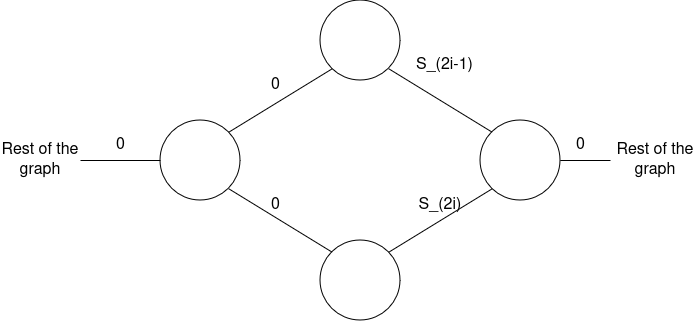
\includegraphics[width=0.6\linewidth]{Latex/Billeder/PBPToMFMST.png}
    \caption{How $(s_{2i-1},s_{2i})$ is modeled in our graph input}
    \label{fig:PBPToMFMST}
\end{figure}

The module or subgraph shown in figure \ref{fig:PBPToMFMST} is repeated for each pair $(s_{2i-1},s_{2i})$ and these subgraphs are connected together. We will show how this is done for the example input to PBP $(1,4,5,8)$. This is seen in figure \ref{fig:PBPToMFMSTExample}. 

\begin{figure}[h]
    \centering
    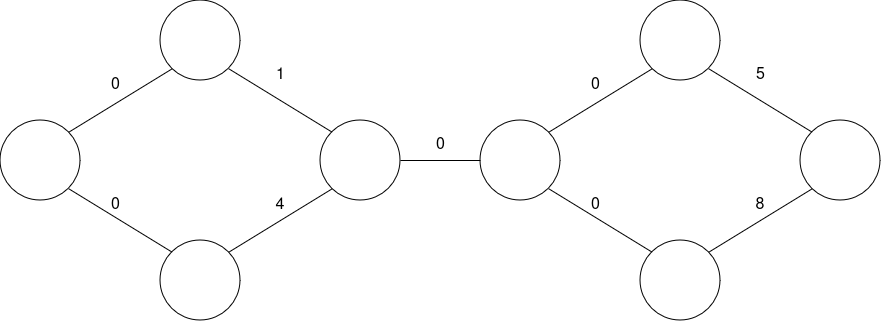
\includegraphics[width=0.6\linewidth]{Latex/Billeder/PBPToMFMSTExample.png}
    \caption{The MFMST transformation of the PBP input $(1,4,5,8)$}
    \label{fig:PBPToMFMSTExample}
\end{figure}
In the following we will identify the edge corresponding to the number $s_i$ simply as the edge $es_i$ and we will refer to the set containing these edges $ES$. 
\\
So to transform a PBP problem to MFMST we create a weighted graph as presented above and then we set $S=\sum_{i=1}^{2n}s_i$ and finally $B=\frac{S}{2}$. We then pair the edges such that $es_{2i-1}$ is paired with $es_{2i}$ and the edges with weight 0 are paired arbitrarily. This we do by constructing the edge sequence $E=\Big(es_1,es_3,\dots,es_{2n-1},\text{all the other 0 weight edges},es_{2n},es_{2n-2},\dots,es_{2}\Big)$. Since the size this graph is linear in the size of the input to PBP, it is clear that this transformation can be performed in polynomial time.

\subsection*{We never include the both the edge $es_{2i-1}$ and $es_{2i}$ in our spanning tree}
We will first argue that any solution to our MFMST transformation will not select both the edge $es_{2i-1}$ and $es_{2i}$. First we can see from figure \ref{fig:PBPToMFMST}  that any solution must include at least $s_{2i-1}$ or $es_{2i}$ in the spanning tree. So the spanning tree contains at least $n$ edges corresponding to our input numbers. \\
Now assume that for some $j\in [1..n]$ that both $es_{2j-1}$ and $es_{2j}$ are in our solution $ST$. We know that $\sum_{e\in ST} w(e) = \sum_{e\in ST\cap ES} w(e) \leq \frac{S}{2}$, but since every $es_i$ not in $ST$ is in the mirror of $ST$ we also know that $\sum_{e\in ES\backslash ST}w(e) \leq \frac{S}{2}$. Clearly the sets $ST \cap ES$ and $ES \backslash ST$ form a partition of $ES$. So the sum of all the weights of their edges is exactly $S$. Therefore the only way both $\sum_{e\in ST\cap ES} w(e) \leq \frac{S}{2}$ and $\sum_{e\in ES\backslash ST}w(e) \leq \frac{S}{2}$ can be true is if 
$\sum_{e\in ST\cap ES} w(e) = \frac{S}{2}$ and $\sum_{e\in ES\backslash ST}w(e) = \frac{S}{2}$ hold. This however leads to a problem. Since both $es_{2j-1}$ and $es_{2j}$ are in $ST$ they are also both in the mirror of $ST$. Therefore the sum of weights in the mirror becomes $(\sum_{e\in ES\backslash ST} w(e)) + s_{2j-1} + s_{2j} = \frac{S}{2} + s_{2j-1} + s_{2j}$. As every $s_i$ is a natural number we get that $\frac{S}{2} + s_{2j-1} + s_{2j} > \frac{S}{2}$. This means that our solution $ST$ is not a valid solution and our assumption that both $s_{2j-1}$ and $s_{2j}$ were in $ST$ was false. So we conclude that for all $i\in[1..]$ any solution $ST$ contains either $es_{2i-1}$ or $es_{2i}$.

\subsection*{PBP reduces to MFMST}
Now that we have our transformation from PBP to MFMST and we have proved some additional things we can show that our transformation indeed is valid and therefore PBP $\leq_p$ MFMST in the following. 

\subsubsection*{The answer to PBP is YES}

In this case there exists a set $A$ that partitions the numbers $(s_1,s_2,\dots, s_{2n})$ such that $\sum_{i\in A} s_i = \sum_{i\in\{1..2n\}\backslash A } s_i$. From this we easily get 
\begin{gather*}
    \sum_{i\in A} s_i + \sum_{i\in\{1..2n\}\backslash A } s_i = \sum_{i=1}^{2n} s_i \Leftrightarrow\\
    2\cdot\left( \sum_{i\in A} s_i \right) = \sum_{i=1}^{2n} s_i \Leftrightarrow\\
    \sum_{i\in A} s_i = \sum_{i\in\{1..2n\}\backslash A } s_i = \frac{\sum_{i=1}^{2n} s_i }{2} 
\end{gather*}

A solution to MFMST transformation is simply the spanning tree $ST$ where we choose the edges $es_i$ such that $i\in A$. As $A$ contains exactly one $i$ from each pair $(2j-1,2j)$ for $j\in[1..n]$ we know that our tree includes exactly one of the edges $es_{2j-1}$ and $es_{2j}$ for $j\in [1..2n]$. By adding all the edges in the graph with weight 0 this is ensured to be a spanning tree. We can now calculate the weight of $ST$ and its mirror.
\begin{gather*}
    \sum_{e_i\in ST} w(e_i) = \sum_{e_i\in ST\cap ES} w(e_i) = \sum_{i\in A} s_i = \frac{S}{2}\\
    \sum_{e_i\in ST} w(e_{m+1-i}) = \sum_{e_i \in ES \backslash ST} w(e_{m+1-i}) = \sum_{i \in \{1..2n\}\backslash A} s_i = \frac{S}{2}
\end{gather*}

As we can see from above both the weight of $ST$ and its mirror are less than or equal, in this case equal, to $\frac{S}{2}$ which was our chosen $B$. Therefore the answer to MFMST is also YES.

\subsubsection*{The answer to MFMST is YES}
If the answer to MFMST is YES we have a spanning tree $ST$ such that the following holds.
\begin{gather*}
    \sum_{e_i\in ST}w(e_i) \leq \frac{S}{2} \land \sum_{e_i\in ST} w(e_{m+1-i}) \leq \frac{S}{2}
\end{gather*}
However as we have argued earlier $ST$ essentially partitions the edges in $ES$. The set $ST$ contains exactly $n$ edges from $ES$ with exactly one from each pair $(es_{2j-1},es_{2j})$ for $j\in [1..n]$. So we can simplify the above inequalities as follows.
\begin{gather*}
    \sum_{e_i\in ST}w(e_i) = \sum_{e_i \in ST\cap ES} w(e_i) = \sum_{es_i \in ST\cap ES} w(es_i) = \sum_{es_i \in ST\cap ES} s_i \leq \frac{S}{2} \land \\
    \sum_{e_i\in ST} w(e_{m+1-i}) = \sum_{es_i\in ES \backslash ST} w(es_i) = \sum_{es_i\in ES \backslash ST} s_i \leq \frac{S}{2} 
\end{gather*}
We also know that since the sets $ST \cap ES$ and $ES \backslash ST$ partition $ES$ the only way that the sum of their weights both are less or equal to half of the total sum of weights in $ES$ is if each sum is actually equal to exactly half of of the total sum. This means that $\sum_{es_i \in ES\cap ST} s_i = \sum_{es_i\in ES \backslash ST} s_i = \frac{S}{2}$. To find a valid partition in PBP we choose  $A=\{i\mid es_{i} \in ST\}$. We now get
\begin{gather*}
    \left(\sum_{i\in A} s_i = \sum_{es_i\in ST \cap ES} s_i = \frac{S}{2}\right) \land
    \left(\sum_{i\in \{1..2n\}\backslash A} s_i = \sum_{es_i \in ES \backslash ST} s_i = \frac{S}{2}\right) \\ \implies\\
    \sum_{i\in A} s_i = \sum_{i\in \{1..2n\}\backslash A} s_i 
\end{gather*}
Since we know that $ST$ contains exactly one edge in the pair $(es_{2j-1},es_{2j})$ for $j\in[1..n]$ we know that $A$ contains exactly one of the numbers in the pair $(2j-1,2j)$ for $j \in [1..n]$. This combined with result expressed above we can conclude that the answer to PBP is also yes.

\subsection*{PBP $\leq_p$ MFMST}
We have now shown that there exists a polynomial time transformation from PBP to MFMST, such if the answer to PBP is YES so is the answer to the MFMST transformation and if the answer to the MFMST transformation is YES so is the answer to PBP. We can therefore conclude that PBP $\leq_p$ MFMST. Since PBP is $\mathcal{NP}$-complete this means that MFMST is also $\mathcal{NP}$-complete.